

\documentclass[color=usenames,dvipsnames]{beamer}

\usepackage[adobefonts,noindent]{ctex} %中文支持
\setCJKmainfont{SimSun}

\mode<presentation> {

\usetheme{Madrid}
\usecolortheme{lily}
\useoutertheme{infolines}

}


\usepackage{booktabs} 
\usepackage{tikz}


% Thin fonts
\usepackage{cmbright}
\usepackage[T1]{fontenc}

\definecolor{dark_grey}{gray}{0.5}
\setbeamercolor{normal text}{fg=dark_grey,bg=white}
\setbeamertemplate{navigation symbols}{}

\setbeamercolor*{palette primary}{fg=gray!100,bg=gray!10}
\setbeamercolor*{palette quaternary}{fg=gray!100,bg=gray!10}
\setbeamercolor*{palette secondary}{fg=gray!100,bg=gray!20}
\setbeamercolor*{palette tertiary}{fg=gray!100,bg=gray!10}
\setbeamercolor*{navigation symbols}{fg=white,bg=white}
\usefonttheme{default}


\setbeamertemplate{blocks}[rounded][shadow=false]
\setbeamercolor{block title}{bg=gray!10}
\setbeamercolor{block body}{fg=gray,bg=gray!10}
%\setbeamercolor{frametitle}{fg=}

\setbeamertemplate{frametitle}[default][center]

\setbeamertemplate{itemize items}[default]
\setbeamertemplate{enumerate items}[default]

\newcommand{\F}{\mathbb{F}}


\title[Your Short Title]{Your Presentation}
\author{You 韩喆}
\institute{Where You're From}
\date{Date of Presentation}
\begin{document}


\begin{frame}
  \titlepage
\end{frame}

% Uncomment these lines for an automatically generated outline.
%\begin{frame}{Outline}
%  \tableofcontents
%\end{frame}

\section{Introduction}

\frame{
  \begin{columns}[c]
   \column{.15\hsize}
   \column{.7\hsize}
   \begin{block}{}
    \centering \Large 英配中程序  \\ 
    \small --- 标准英文段落/句子生成
   \end{block}
   \column{.15\hsize}
  \end{columns}
}
\begin{frame}{Introduction}

\begin{itemize}
  \item Your introduction goes here! 是韩喆
  \item Use \texttt{itemize} to organize your main points.
\end{itemize}

\vskip 1cm

\begin{block}{Examples}
Some examples of commonly used commands and features are included, to help you get started.
\end{block}

\end{frame}

\section{Some \LaTeX{} Examples}

\subsection{Tables and Figures}

\begin{frame}{Tables and Figures}

\begin{enumerate}
\item Use \texttt{tabular} for basic tables --- see Table~\ref{tab:widgets}, for example.
\item You can upload a figure (JPEG, PNG or PDF) using the files menu. 
\item To include it in your document, use the \texttt{includegraphics} command (see the comment below in the source code).
\end{enumerate}

% Commands to include a figure:
%\begin{figure}
%\includegraphics[width=\textwidth]{your-figure's-file-name}
%\caption{\label{fig:your-figure}Caption goes here.}
%\end{figure}
\
\begin{table}
\label{tab:widgets}
\caption{An Example table}
\begin{tabular}{l l l}
\midrule
Apples & 1 & 2 \\
\midrule
\color{Green}Oranges &\color{Green} 3& \color{Green}4
\end{tabular}
\end{table}



\end{frame}

\subsection{Mathematics}

\begin{frame}{Readable Mathematics}

Let $X_1, X_2, \ldots, X_n$ be a sequence of independent and identically distributed random variables with $\text{E}[X_i] = \mu$ and $\text{Var}[X_i] = \sigma^2 < \infty$, and let
$$S_n = \frac{X_1 + X_2 + \cdots + X_n}{n}
      = \frac{1}{n}\sum_{i}^{n} X_i$$
denote their mean. Then as $n$ approaches infinity, the random variables $\sqrt{n}(S_n - \mu)$ converge in distribution to a normal $\mathcal{N}(0, \sigma^2)$.

\end{frame}


\begin{frame}

\frametitle{Slide 1}
\pause
\begin{block}{Goal}
Main goal that we want to prove.
\end{block}
\pause

\begin{itemize}
\item \color{RedOrange} Something.
\pause
\item \color{Green}
 Something more.
\pause
\item and more!.
\end{itemize}
\pause

\begin{block}{Relaxed Goal}
relaxation
\end{block}
\end{frame}

\begin{frame}
\frametitle{NAE PCP Verifier from Label Cover}
\framesubtitle{using Long Code Reduction}

\begin{columns}[c] % The "c" option specifies centered vertical alignment while the "t" option is used for top vertical alignment
\column{.45\textwidth} % Right column and width
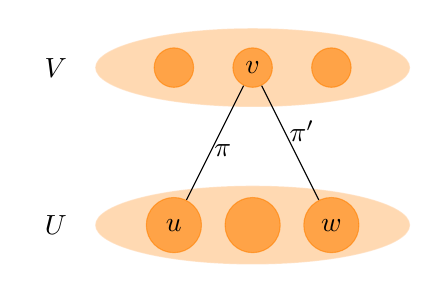
\begin{tikzpicture}[auto,every node/.style={draw=black,circle,inner sep=0pt,minimum size=1cm}]
    \draw[fill=orange,opacity=.3,draw=white] (0,-4) ellipse (2cm and 0.5cm);
    \draw[fill=orange,opacity=.3,draw=white] (0,-2) ellipse (2cm and 0.5cm);


    \node[minimum size=0.7cm,draw=white] at (-2.5,-4) (U) {$U$};
    \node[minimum size=0.7cm,draw=white] at (-2.5,-2) (V) {$V$};

    \node[minimum size=0.7cm,fill=orange,opacity=.6, text opacity=1,draw=orange] at (-1,-4) (nodeU) {$u$};
    \node[minimum size=0.7cm,fill=orange,opacity=.6, text opacity=1,draw=orange] at (1,-4) (nodeUp){$w$};
    \node[minimum size=0.7cm,fill=orange,opacity=.6, text opacity=1,draw=orange] at (0,-4) (nodeUpp){};

    \node[minimum size=0.5cm,fill=orange,opacity=.6, text opacity=1,draw=orange] at (-1,-2) (nodeVpp){};
    \node[minimum size=0.5cm,fill=orange,opacity=.6, text opacity=1,draw=orange] at (0,-2) (nodeV){$v$};
    \node[minimum size=0.5cm,fill=orange,opacity=.6, text opacity=1,draw=orange] at (1,-2) (nodeVp){};

\path (nodeV) edge  node [minimum size=0cm,draw=white,opacity=0,text opacity=1] {$\pi$} (nodeU) ;
\path (nodeV) edge  node [minimum size=0cm,draw=white,opacity=0,text opacity=1] {$\pi'$} (nodeUp) ;

\end{tikzpicture}

\pause
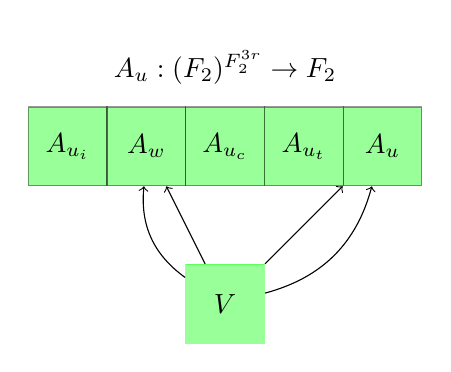
\begin{tikzpicture}[auto,every node/.style={draw=white,circle,inner sep=0pt,minimum size=1cm}]
   \node[rectangle,minimum size=0,inner sep = 0pt,draw=white] at (0,1.5) (B) {};
   \node[rectangle,minimum size=0,inner sep = 0pt,draw=white] at (0,1) (A) { $A_u:(\F_2)^{\F_2^{3r}} \rightarrow \F_2$};

   \node[rectangle,inner sep = 2pt,fill=green,opacity=.4, text opacity=1,draw=green] at (0,-2) (V) {$V$};

    \node[rectangle,fill=green,opacity=.4, text opacity=1,draw=black] at (-2,0) (Aui) {$A_{u_i}$};
    \node[rectangle,fill=green,opacity=.4, text opacity=1,draw=black] at (-1,0) (Auj) {$A_{w}$};
    \node[rectangle,fill=green,opacity=.4, text opacity=1,draw=black] at (0,0) (Auc) {$A_{u_c}$};
    \node[rectangle,fill=green,opacity=.4, text opacity=1,draw=black] at (1,0) (Aut) {$A_{u_t}$};
    \node[rectangle,fill=green,opacity=.4, text opacity=1,draw=black] at (2,0) (Aus) {$A_{u}$};

 \path    (V) edge [->, bend left]   (Auj)  edge [->]   (Auj)         edge  [->]      (Aus) edge [->,bend right]    (Aus);



\end{tikzpicture}



\column{.55\textwidth}\pause % Left column and width
\begin{itemize}

\item Query 
\begin{enumerate}
\item $A_u(e),A_u(e+ f\circ \pi + 1+\eta)$
\item $A_w(e'),A_w(e'+f\circ \pi'+ \eta')$
\end{enumerate}
\item Where 
\begin{enumerate}
\item $e,e' :\F_2^{3r} \rightarrow \{0,1\}$,  $f :\F_2^{r} \rightarrow \{0,1\}$
\item $\eta,\eta'$ from noise distribution.
\end{enumerate}
\pause
\item Correct proofs are Long Code encodings of labels to $U$ given by
$$A_u = (f(a))_{f \in  (\F_2)^{\F_2^{3r}}}$$
\end{itemize}\pause
\center{\alert{\textbf{Bottleneck! : } Proof size is $2^{2^{3r}}n^r$. \\Cannot go beyond $r = O(\log \log n)$.}}
\end{columns}
\end{frame}



\end{document} 